\documentclass[conference]{IEEEtran}
% \IEEEoverridecommandlockouts
% The preceding line is only needed to identify funding in the first footnote. If that is unneeded, please comment it out.
\usepackage{cite}
\usepackage{amsmath,amssymb,amsfonts}
\usepackage{algorithmic}
\usepackage{hyperref}
\usepackage{graphicx}
\usepackage{textcomp}
\usepackage{xcolor}
\def\BibTeX{{\rm B\kern-.05em{\sc i\kern-.025em b}\kern-.08em
    T\kern-.1667em\lower.7ex\hbox{E}\kern-.125emX}}
\begin{document}

\title{Computer Technology Project I\\}

\author{\IEEEauthorblockN{Simon Nyman}
\IEEEauthorblockA{\textit{Dept. of Electrical and Computer Engineering} \\
\textit{Aarhus University}\\
Student number: 202305077\\}
\and
\IEEEauthorblockN{Jakob Palm}
\IEEEauthorblockA{\textit{Dept. of Electrical and Computer Engineering} \\
\textit{Aarhus University}\\
Student number: 202307244\\}
}

\maketitle

\begin{abstract}
    This report documents the development of a Search and Rescue robot designed on a Turtlebot3 using the ROS framework along with several external software and hardware components.
    Throughout the report, the specifics of these components will be introduced along with the thought process behind the implementation.

    As the nature of the robot is Search and Rescue, the overall aim of the project is to find as many victims as possible while avoiding obstacles.
    The main focus of ours, was the development of the navigational software, which will be be explained in depth with the use of figures and the like, all aiming to clarify and explain the process of the algorithm as clearly as possible.
    We will go in depth with how we conducted experiments, and the importance of our testing process guiding us towards good solutions.
    Genereally, we reached a fairly well working implementation, though with a few weaknesses and sources of error, which will be discussed in depth over the course of the paper.
    Furthermore we will dive into the reasoning behind our design decisions, along with a discussion and reflexion on what improvements could have been made.

    At last we conclude that we achieved our goals and...
    Overall we acquired some foundational tools for future robot developing and the computer engineering field as a whole.
\end{abstract}

\section{Introduction}
The goal for this project was to design a down-scaled version of a Search And Rescue (SAR) robot, used to rescue victims in the aftermaths of natural disasters.
The robot will imitate a real world scenario by autonomously navigating an obstacle course and distinguishing between different color markings, representing potential victims. To achieved this we use the TurtleBot3 Burger Robot equipped with different sensors.
All the software will be implmented in python using the Robot Operating Software framework (ROS). For the sensors we will be using a LiDAR sensor capable of measuring distances in a 360 degree view, and an RGB-sensor which differentiates between red, green, and blue colors. 
The overall structure of the project was split into four parts:
\begin{itemize}
    \item Understanding the basic concepts of robotics programming, including the see-think-act cycle \href{sec:STAC}{Fig. 1}. Reading and processing data from a RGB and range sensor.
    \item Setting up a virtual machine, and working with ROS through a beginner's tutorial.
    \item Developing the robot navigation program, and working with ROS on the Raspberry PI .
    \item Optimizing the robot navigation and integrating code components for the RGB and LEDs
\end{itemize} 
Finally, the performance of the robot would be assessed based on three factors: Average speed, number of collisions and "victims" found.
In this report we will firstly go through the specifications for the hardware and software that was used.
Thereafter we will elaborate on the methods used for implementing the different parts of the project.
Then we will explain how we used experimentation and testing throughout the course, and what findings were made.
At the end we will discuss the upsides and downsides of our approach, followed by a conclusion where we evalute the process as a whole.

\section{Specifications}
Our Search and Rescue implementation used a turtlebot3 robot, specifically the burger configuration with dimensions 138mm x 178mm x 192mm (L $\times$ W $\times$ H)\cite{b1}.
On the turtlebot3, a Raspberry Pi 3 model B+ and an Arduino are connected in order to process the incoming external signals from the various sensors.
Furthermore, the robot has two motors attached, one for each wheel. From the specification it is evident that the robot has a maximal linear velocity of 0.22 m/s
and a maximum rotational velocity of 2.84 rad/s. In order keep the robot as agile as possible with no wires attached, we used an 800 mA Li-Po battery and established a wireless connection, which will be specified further in a following section.
The specific RGB used is an ISL29125 low power, high sensitivity red, green and blue light sensor with SMBus compatibility\cite{b2}.
The LiDAR used is the LDS-01 version with a range of 120 mm to 3500 mm, capable of doing full 360 degree scans. \cite{b3}

\subsection{Software Setup}

\subsubsection{Network Configuration}
As mentioned, we wanted the robot to be able to move as freely as possible, meaning that connecting it to our machine via an ethernet cable was not the way to go.
Therefore, we established a wireless connection to the robot by changing the network configuration on the sd card, making it automatically connect to the IP-address of our machine.
This allowed for easy connection to the robot once a mobile hotspot was opened, as the robot was automatically allocated an IP-address.
With this configured, the robot would subscribe to our machine on which the required ROS environments (these will be specified in the next section) would publish actuation data to the motors of the robot, enabling wireless navigation.

\subsubsection{ROS}

The ROS operating system proved to be very useful in regards to this project, as it provided a greatly practical and convenient framework for our specific problem.
The three main parts used were topics, messages, and nodes (rostopic, rosmsg, rosnode). These are all integral parts of the ROS framework, as each provides a unique functionality in abstracting the navigation.
Nodes are responsible for performing computations and communicate internally through topics, while messages are used for communicating with the external sensors.

In our case, we had three nodes running. One running roscore, which encapsulates the entire framwork, allowing the other nodes to run in the ROS environment.
The second node ran the basic functionality of the robot, such as managing the incoming sensor data and sending signals to the motors, while the third node was used to run our navigation code.
These communicated by the subsribe/publish model to send data back and forth, in order to control the navigation of the robot.
Another beneficial characteristic of the ROS nodes is that they also contain debug information and data. This allowed for logging the information required for optimizing and reasoning about the relevant aspects of the code as it was being tested.

\section{Methodology and Design}
Throughout the project we have been using the trial and error approach, which allowed for an efficient overall workflow. 
This approach works well when having to build and optimize code for hardware, instead of reasoning about it on an abstract level, which would only get us so far, since we are beginners in this field.
With this approach we would be able to instantly see if and how the code is working.
Furthermore, this approach works in great synergy with the See-Think-Act Cycle we use for the robot, see \href{sec:STAC}{Fig. 1}.
We are able to edit the "see", "think" and "act" parts individually and get instant feedback by testing. 
This approach to navigation is very straight forward to reason about, simplifying both the building and optimization processes.
For the implementation of this design we developed an algorithm, capable of navigating an arbitrary obstacle course, while checking for victims and collisions.
This happens through a loop that runs continually until a desired duration is reached or terminated by user input. 
\begin{figure}[htbp]
    \centerline{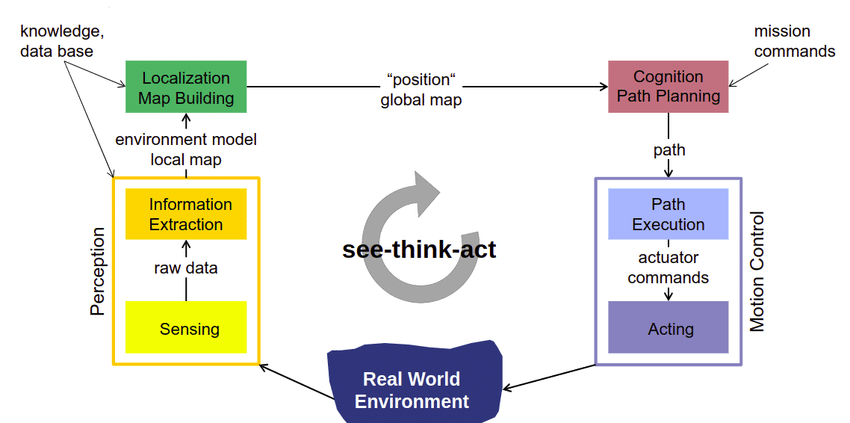
\includegraphics[width=1.0\columnwidth]{Pictures/STAC.png}}
    \caption{Robots See-Think-Act Cycle.}
    \label{sec:STAC}
    \end{figure}

\subsection{LiDAR}
The use of LiDAR readings is an integral part of the design, as the entire navigation logic depends upon these.
In our implementation, it had two use cases, one being the ability to read in which direction the nearest obstacle was present, if any, and the second being the ability to read the specific distance to said obstacle, which would determine what to do next.

As the LiDAR provides a 360 degree scan, we first had to figure out which angles to use and how these were organized within the data provided by the LiDAR.
By firstly playing around with the angles, we figured out that they were organized in a way such that 0$^\circ$ was at the back of the robot, and then continued clockwise around the robot.
This meant that the front 180$^\circ$ were located in the interval $[90:270]$. How this was used in our final implementation will be elaborated on in the \textit{Navigation} section.

During initial testing of the LiDAR, we encountered a problem, as some angles seemed to not be working properly and would either give readings very close to 0, which resulted in the robot refusing to move, or infinitely large readings.
To fix this, we wrote a loop within the LiDAR scan function, which would iterate through the values in the angles being read and, if any angles were suffering from either of these problems, would fix them, as seen in \href{sec:lidar}{Fig. 2}.
If the value was infinitely large, it would set it to the max value of the LiDAR, which, as previously mentioned, is 3.5 meters.
In the case that an angle gave readings very close to 0, it would set this to 1 meter as this would have no impact on the other readings.
We had a third case, which checked whether the reading was indeed a number as it should, and would otherwise set it to 0 in which case it would be ignored as described.
With this configured, we additionally addded a few centimeters to each reading due to the innate imprecision of the LiDAR, which will be apparent later on.
\begin{figure}[htbp]
    \centerline{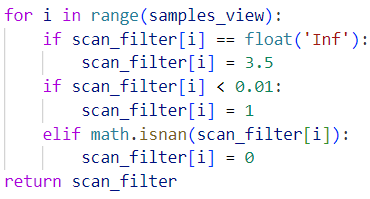
\includegraphics[width=0.6\columnwidth\hspace{-1.3cm}]{Pictures/LiDARhvid.png}}
    \caption{Ignoring the dead LiDAR angles.}
    \label{sec:lidar}
    \end{figure}

\subsection{Navigation}
The logic for the navigation was developed to excel on our performance criteria of limiting collisions, while achieveing a high speed, which in turn will allow the robot to move fast through the obstacle course, thereby detecting as many "victims" as possible.
Our navigation is based on an object detecting strategy, were we made the robots actions dependent on where the closest object was located.
To distinguish between possible locations of an object, we had to split the LiDAR readings into both an angular interval and distance intervals.
For our final iteration of the navigation program, we split the angular intervals into 6 cones, each spanning 25 deegrees in front of the robot as illustrated in \href{sec:angles}{Fig. 3}. 
As the navigation is based around the concept of avoiding objects obstructing the path of the robot, we chose to "ignore" the 180 deegrees behind the robot. 
We did this by programming, that if an obstacle was the detected in those angles the robot should move forward in full speed.
The same concept is applied to the two remaining 15 deegree cones of the forward facing 180 deegrees, which enables the robot to run parralel to an object without turning away.
\begin{figure}[htbp]
    \centerline{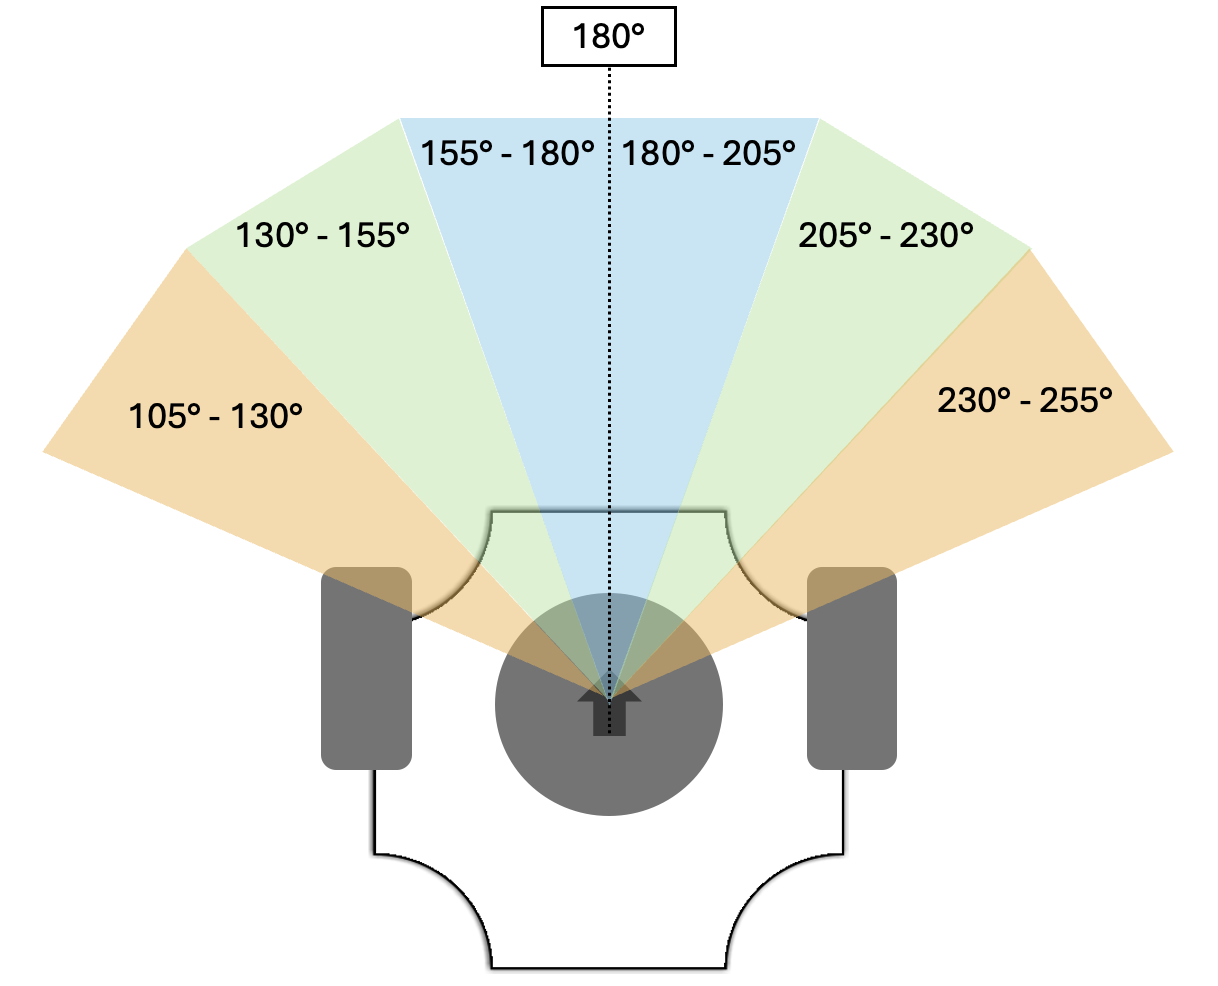
\includegraphics[width=0.9\columnwidth]{Pictures/LiDAR Angels.png}}
    \caption{LiDAR zones illustration. Please note that the angles of the cones are slightly distorted}
    \label{sec:angles}
    \end{figure}
When the the angle interval of the nearest object is registered, the navigation program would then evaluate the distance to the obstacle.
If the obstacle is registered to be within 30 centimeters, the robot would make a slight preventive turn while keeping the linear speed high.
If the object is within 22 centimeters, the robot would turn hard while lowering the linear speed drasticly.
In addition to that if an obstacle should be registered within 10 centimeters of the LiDAR, a collision would be registered.
An illustration of the distances within the cones is provided in \href{sec:distances}{Fig. 4}.
The intervals and distances were both determined through our continuous testing process, which we elaborate further on in the \textit{Experimentation and Testing} section.
\begin{figure}[htbp]
    \centerline{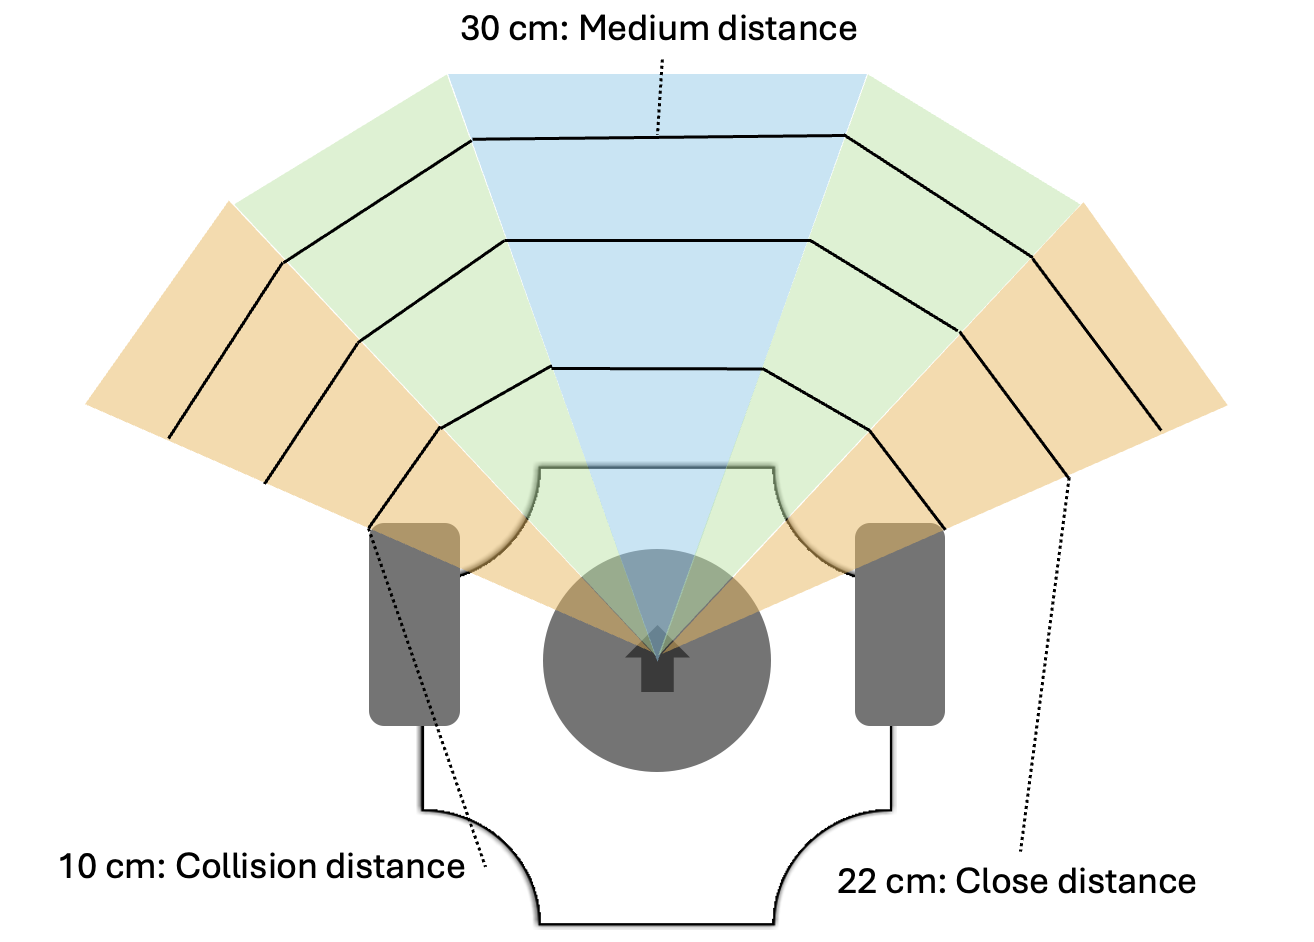
\includegraphics[width=0.9\columnwidth]{Pictures/LiDAR Distances.png}}
    \caption{LiDAR distances illustration. Please note that the angle of the cones and distances are slightly distorted}
    \label{sec:distances}
    \end{figure}

The thought behind this approach to our logic design, was to use the medium distance to locate objects early and then make the robot take preventive action.
Locating the obstacles early allows the robot to make a series of smaller turns, where the linear speed is kept high. The concept is visualized in \href{sec:medium aviodance}{Fig. 5}.
The close distance was implemented to be used in situations where harder turns were needed to avoid a collision. A potential example could be a dead end, as illustrated in \href{sec:close aviodance}{Fig. 6}.
\begin{figure}[htbp]
    \centerline{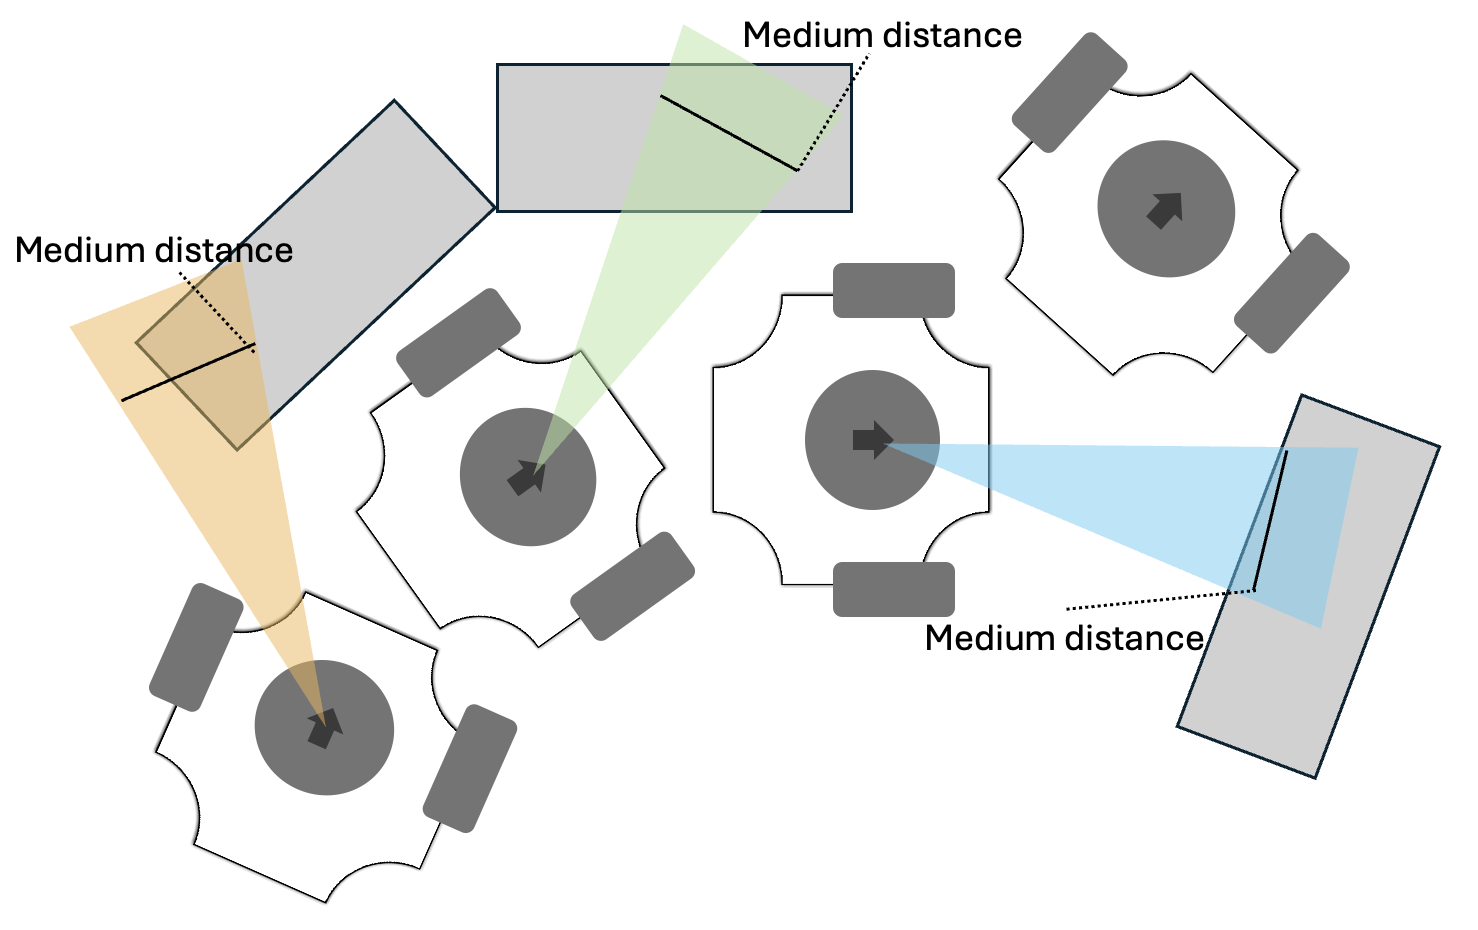
\includegraphics[width=0.9\columnwidth]{Pictures/Medium Distance Aviodance.png}}
    \caption{Illustration of the robot using the medium distance in different angle intervals to move fast through a potential obstacle course scenario.}
    \label{sec:medium aviodance}
    \end{figure}
\begin{figure}[htbp]
    \centerline{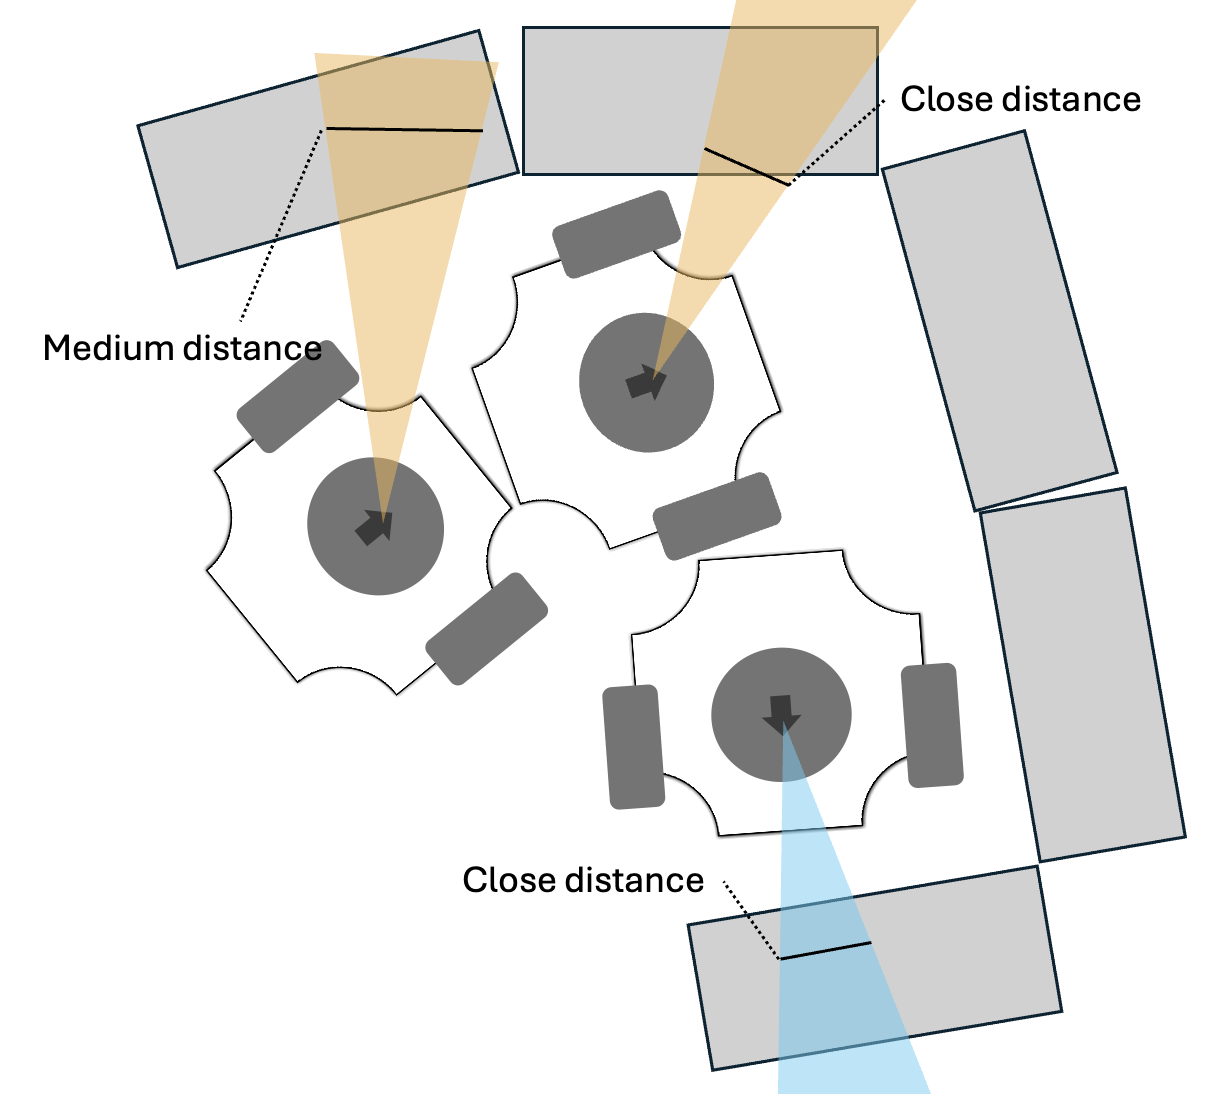
\includegraphics[width=0.9\columnwidth]{Pictures/Close Distance Avoidance.png}}
    \caption{Illustration of a scenario where the robot would use the close distance.}
    \label{sec:close aviodance}
    \end{figure}

The way we implemented this navigation logic is illustarated by the flow chart in \href{sec:flowchart}{Fig. 7}. 
First we would locate if there is an obstacle in our LiDAR zones, if not the robot would continue moving forward.
If an obstacle was detected, it would be evaluated in which cone, and thereafter at what distance.
If the obstacle was in either of the center cones, it would mean the obstacle is diretcly in the robots path meaning the robot will have to turn a lot.
The robot will have to turn less if an obstacle was detected in the middle cones, and even less if the obstacle was in the outer cones.
For the distance factor, an obstacle within the medium distance would result in maximum linear speed, but a close obstacle would mean a very significantly reduced linear speed.

To summarize, the angle of the obstacle relative to the robot would be the primary factor in determining the angular speed (i.e how much the robot turns), so the closer an obstacle is to the current path of the robot, the more it will turn.
In addition to that, the distance to said obstacle would be the primary factor in determining the linear speed (i.e how fast the robot moves forward), so the closer an obstacle is to the robot, the slower it will move to avoid collisions.
\begin{figure}[htbp]
    \centerline{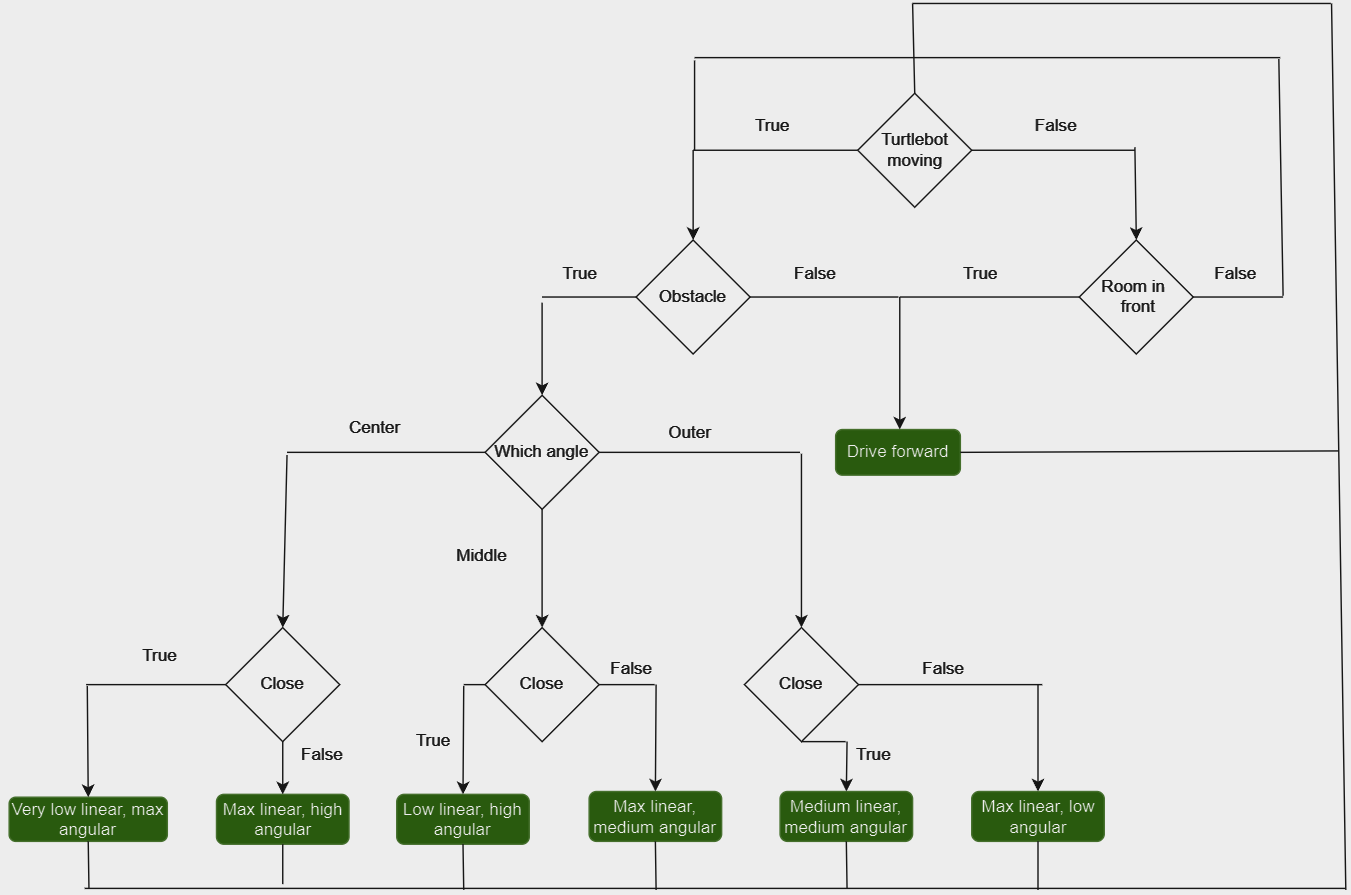
\includegraphics[width=1.0\columnwidth]{Pictures/Flowchart.png}}
    \caption{Flowchart describing how the robot will act, depending on relative position of obstacle.}
    \label{sec:flowchart}
    \end{figure}

For the conrete implmentation we would use a bunch of if- and else statements, ressembeling the pseudo code in \href{sec:pseudo}{Fig. 8}.
The first set of if statements would determine in which angle the closest obstacle was present.
Thereafter some nested if statements would determine how far the object was from the robot.
We would then through our testing find the best combination of linear and angular speed, to achieve the desired action.
For example in \href{sec:navigation}{Fig. 9} a snippet of our navigation code is provided, where one of the front cones are being evaluated. 
Here the combination og linear and angular, when registering a object at a close distance, will resemble an almost full u-turn when executed.
\begin{figure}[htbp]
    \centerline{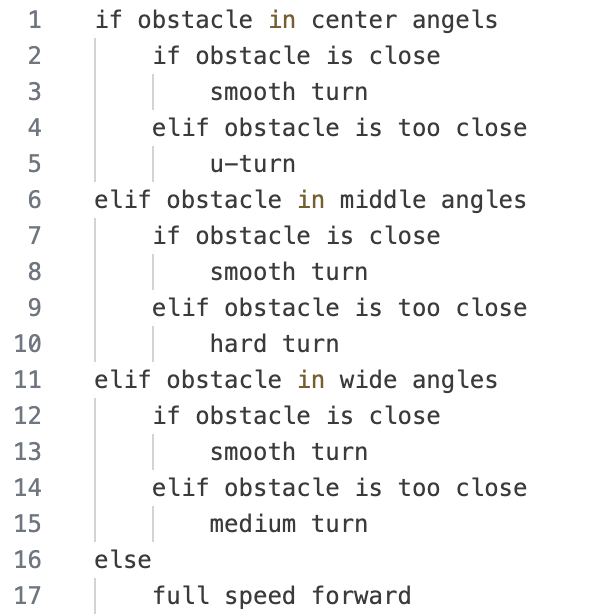
\includegraphics[width=0.6\columnwidth\hspace{-1.3cm}]{Pictures/Pseudo.png}}
    \caption{Pseudo navigation code.}
    \label{sec:pseudo}
    \end{figure}
\begin{figure}[htbp]
    \centerline{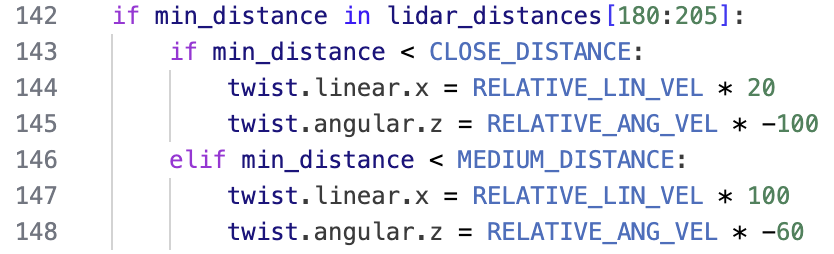
\includegraphics[width=0.9\columnwidth\hspace{-0.1cm}]{Pictures/Navigation.png}}
    \caption{Navigation code snippet.}
    \label{sec:navigation}
    \end{figure}  
\subsection{RGB}
As the point of the robot was to Search and Rescue, we needed a way to detect when a victim was found, which was done by the aforementioned RGB sensor, as the victims were represented by red spots on the floor.
With this in mind, we placed the RGB sensor as close to the ground as the robot allowed for in order to keep the readings as centralized as possible.
Additionally, we also connected a white LED and placed it directly next to the RGB sensor as we experienced that it had some trouble distinguishing between colors if not properly lit.
The RGB was connected to the Raspberry Pi using four pins, two of these being the SDA (Serial Data Line) and SCL (Serial Clock Line)\cite{b4}. The SDA is the pin resposible for transfering raw data from the sensor to the Pi, where it is interpreted processed in order to extract the red, green, and blue values.
The SCL is simply a clock, which synchronizes data transfers over the I2C bus.

Furthermore, the sensor was connected to a GPIO pin, which would provide power to the RGB when the code was executed, with the fourth pin simply being ground.
After connecting the RGB properly, we were able to read the different values at the clock rate provided by the SCL.
Since the victims were represented by red dots, we wrote our code in such a way that it would find a victim each time the red readings were above a certain threshold.

However, due to unavoidable uncertainties in measurement, we would have to manually upscale the blue readings by a certain factor as these seemed to consistently be a bit lower than expected.
This was done by simply isolating the blue data and multiplying it by a factor we found fitting.
Eventually, the condition for finding a victim was as shown in Fig. 9.
If all these conditions were met, an LED would light up and our \textit{victim counter} variable would be incremented by 1.
With the detection code finished, a short delay was added to the detection as the sensor would otherwise be able to detect multiple victims from a single red spot, courtesy of the high clock speed.

\begin{figure}[htbp]
    \centerline{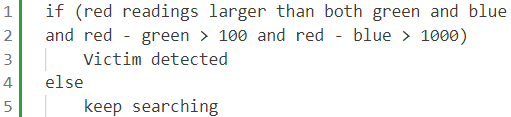
\includegraphics[width=0.9\columnwidth]{Pictures/rgbpseudo.png}}
    \caption{pseudo code showcasing the RGB logic.}
    \label{sec:rgb}
    \end{figure}

\subsection{LED}
As mentioned in the RGB section, we had an LED light up each time a victim was found. This was done by simlpy connecting it to a different GPIO than the RGB and then having it light up whenever the victim conditions were met.
It would light up for a set amount of time and then turn off again afterwards.

The same thing was done for the \textit{collision counter} variable, as this was also signified by an LED, only in a different color.
This would light up whenever the robot received a reading from the LiDAR below a certain threshold, corresponding to the length of the robot.
Again, the LED would light up for a short amount of time while also incrementing the variable responsible for counting the total amount of collisions during a run.
This detection was implemented completely independent from the other navigation code, resulting in us being able to detect a collision regardless of what stage of navigation the robot was currently in.

\section{Experimentation and Testing}
As mentioned earlier we have been constanly running tests throughout the course, in order to figure out what works and what does not.
The testing and experiments consisted mostly of figuring out how we wanted the robot to respond to a given scenario, then creating that scenario and evaluting what actually happend.
We focused on testing in order to shorten the feedback loop, and get respons on what we would have developed.
Throughout the course it was confirmed to us that this was the right approach, as the best results came when we tested smaller changes at a time.
As we would be running a lot of tests, it was important for us to make the testing process as smooth as possible.
As mentioned in \textit{Navigation} the main parameters our overall strategy allowed us to adjust, was how we would divide the LiDAR readings into different angle and distance intervals, and then what linear and angular speed the robot should move with.
To make these parameters easily adjustable, we introduced them as global variables, except for the angular divison of the LiDAR readings, which we elaborate on later.
For for the speeds of our robot we found the maximum linear speed to be 0.22 meters per second, and the maximum angular speed to be 2.84 radians per second.
By dividing each of these by a 100, we got a relative velocity for both, allowing us to adjust how many percent of the maximum speed we wanted to use.
Furthermore, for the distances we simply just created global variables, which would be used in the navigation part of the code.
As to why the same was not done for the angular division, it came down inconvenience.
We would experiment with a bunch of different setups, both changing the size and amount of cones used, which did not suit the use of global variables for the sake of adjustability.

Through our testing we found the following to be the optimal setup:

As mentioned earlier, we split the angular intervals into 6 cones, each spanning 25 deegrees in front of the robot as illustrated in \href{sec:angles}{Fig. 3}.
We found this to be optimal beacause; when we went for smaller intervals, either the obstacle would not register, causing a collision, or it would register in different cones when testing the same scenarios, causing inconsistensy.
On the other hand when we went for larger intervals, we would have to generalize the action of the robot, meaning that one cone would have to account for multiple scenarios, which hurt our speed.

And for the distances within those cones we differentiated between obstacles within 30 centimeters and 22 centimeters, as mentioned before and seen in \href{sec:distances}{Fig. 4}.
Again we found this to be optimal beacause; adding more distances resulted in collisions, which was due to the see, think, act cycle of the robot took some time to execute.
We found that before the robot had "registered" the obstacle (see), to then process the information (think) and then act, the robot would have moved into a diffrent distance zone, often time leading to a collision.
So we got better results primarily using a medium distance for high speed preventive turns, and a close distance to get out of more tricky situations.

Finally, for our linear and angular speeds, we simply just fine tuned the values to achieve our overall goal of moving as fast as possible to cover the most ground, while getting as close to the obstacles as possible without colliding.

The whole testing en experimentation process

With all of this combined we were able to achieve our goal of designing a dwon-scaled version of a search and rescue robot, with the ability to autonomously navigate.
Furthermore we also achieved our goal of performing well, in regards to our performance criteria of moving at a high average speed while avoiding collisions and detecting as many victims as possible.

\section{Discussion}
Throughout the project, we rigorously tested the program and attempted more complex iterations than what ended up being our final implementation.
However, we discovered that often simplicity was the way to go as the course which the robot was going to navigate was not littered with complex obstacles that required sofisticated decision making.
This meant that when we would try out more intricate navigation code, it often led to an ineffeiciently running robot as it was equipped with solutions to a problem that would never arise.
That being said, of course our code was far from perfect and could have been optimized in a manner of ways, but our lack of experience with ROS and robot navigation was evidently a limiting factor in this regard.

By looking at our code afterwards, we discovered a few places in which the code could have been optimized in order for the robot to navigate the course much smoother.
One of such is the hard coded LiDAR angles which the robot uses for navigation. For an uninitiated reader of our code, this may have been a very difficuilt part of the code to make sense of, as they were all written in the form $[index \hspace{1mm} 0: index \hspace{1mm} 1]$.
A much more streamlined and easy to use apporach would have been to make these variable and name them as had been done with many of our other variables used.
This leads to another point of optimization, as we ended up with a messy plethora of different variables, both global and local, which even confused us at times. These could likely have been streamlined and organized much more appropriately, had we been more careful in our naming and organization of these from the beginning.
Additionally, the overall structure of the final program is not ideal as it is constructed in a very blocky manner with a lot of nesting being a clear trend. As we also discovered during our testing process, this makes the code more strenuous to edit as we end up with a lot of unintentional dependencies.

Generally, the soures of error mentioned above all stem from our lack of experience in working on such projects. Especially the monolithic structure of the code means that scalability and maintainability suffers, which is also one of the main difficulties that we encountered.
The frequent hardware interactions and I/O calls all lead to an ineffeiciently running code as these are very time consuming operations.

Had we been able to redo the project, we would likely have used a different approach.
Having a clear plan from the beginning of the project would greatly benefit the development flow of the project as this could likely have avoided many of the errors discussed, since a more streamlined code could have been developed from the very beginning.
This would likely eliminate the repetitive use of nested functions and inefficient hardware communication.
One method could be integrating a bit of machine learning and data storage in the code such that the robot would not visit the same place twice as the course would be mapped along the way. This would greatly improve the efficiency in searching for victims, as we found that often the same victim would be identified multiple times since the robot would return to the point that it was first found, caused by the fact that it had no way of knowing where it had already been.
This approach would definetly benefit our goal of maximum  number of victims found with as high average velocity as possible.
However, in the context of this specific project, this may be overdoing it a bit as the course in which the robot was supposed to run was not very large, but looking at it from purely a search and Rescue point of view, it would definetly be a major improvement.

To optimize purely for the specific course at hand, it might have been a good idea, instead of searching for obstacles, to search for free spaces.
Thinking about this, it becomes apparent that this approach would result in a lighter workload and less data processing, as the direction in which most free space is available is less likely to vary as frequently as the nearest obstacle.
However, it might also result in the robot never reaching certain areas if it is only accessable by a narrow path or similar.

In reflection, we see that our approach definetly had its errors and could have been optimized in many ways that would omit the errors found in our final implementation.
Our approach however still achieves all the goals that we set for ourselves, namely finding as many victims as possible while maintaining a high average speed with as few collisions as possible and we find that in the context of the specific circumstances, the advantages gained from implementing these optimizations would be marginal relative compared to the added complexity.

\section{Conclusion}
Our goal was to implement a SAR robot capable of autonomously navigating an arbitrary obstacle course and locate as many victims as possible.
To achieve this, we aimed for safe and efficient movement through the course.
This was done by utilizing a TurtleBot3 equipped with external sensors along with the highly practical ROS framework and navigational code written in Python.
After establishing a wireless connection to the robot, all these tools enabled the robot to be as agile as possible while synchronously scanning the environment for obstacles and victims, using LEDs to indicate when a victim or collision was registered.

The main algorithm was developed with our methodology in mind, namely the see-think-act cycle in regards to the navigational decision making, which worked in unison with our trial and error approach.
The final iteration used the LiDAR scanner to retrieve data describing the sorrounding environment and thereby allow for efficient movement throughout the course.
The data was then processed by splitting it into six cones and within those cones further distinuish between different distances.
Using this data, the robot would decide how to proceed onward, all the while checking for victims on the ground using the RGB sensor.
In order to account for the different sources of errors, several preventional code was written such that the robot would not react to false readings, whether they were coming from the LiDAR scanner or the RGB sensor.

Through vigorous testing and experimentation, we explored different overall strategies for how to best advance when the robot was presented with obsstacles.
Eventually, we ended up with an object detection and -avoidance strategy which we were able to modify in several ways in order to optimize for the best results.
After going through a long and thorough optmization process, we ended up with our final algorithm, equpped with all the functions needed for the robot to work autonomously and in the end, display the relevant data.

After having developed the program, we were able to reflect on both the final implementation and the process as a whole.
From this, we could conclude that our approach to the project was generally on track with how we would reapproach it, were we able to redo it.
We have discussed several alternative strategies while also reflecting on our own implementation and which weaknesses and strenghts it possesses.
In conclusion, our approach worked well, however with room for improvement, and to achieve these improvements, we would have to adopt a more complex strategy, which in turn would result in marginal gains the amount of added complexity.
The philosophy of keeping it simple but effective is definetly a valid technique, but should the robot have been used in a real Search and Rescue scenario, a more advanced implementation would definetly be required.

Throughout this project, we have acquired very useful experience and several applicable tools in regards to the field of computer engineering as a whole.
Specifically, the process of devising a high level vision for the project and afterwards executing it efficiently on a low level basis.
During this, working with software architecture and the process of testing and experimenting and using the acquired results to improve the given aspects of the project.
Furthermore, we have gained a lot of experience from working with elements and concepts specific to robot development and embedded systems.
Especially using different hardware components such as a LiDAR scanner, an RGB sensor, both having to communicate with the Raspberry Pi mounted on the TurtleBot3.
Also, developing our own python program and executing it using the premade ROS framework has been educational.

\section{Personal Contributions}
Throughout the course, we generally worked in tandem in regards to the development and implementation of the robot.
Whenever a new step had to be taken, we discussed it between the two of us and came up with a rough idea of how to approach the problem and afterwards would work together on the solution, whether it was our navigation software or the integration of a new sensor or other external part.
When writing the report, the workload was divided in the follwing way:

Jakob wrote and was responsible for the following sections:
\begin{itemize}
    \item Section II - Specifications
    \item Subsection II.A - Software Setup
    \item Subsection III.A - LiDAR
    \item Subsection III.C - RGB
    \item Subsection III.D - LED
\end{itemize}

Simon wrote and was responsible for the following sections:
\begin{itemize}
    \item Section I - Introduction
    \item Section III - Methodology and Design
    \item Section III.B - Navigation
    \item Section IV - Experimentation and Testing
\end{itemize}

Sections V and VI along with the Abstract were written in collaboration to achieve a coalescence of thoughts and conclusions.
The same is true for the design of the figures used, along with the gathering of information.
\begin{thebibliography}{00}
\bibitem{b1} 'Turtlebot3 features', accessed 15 May 2024, available at: \url{https://emanual.robotis.com/docs/en/platform/turtlebot3/features/}
\bibitem{b2} 'Renesas RGB-sensor ISL29125 datasheet', accessed 15 May 2024, available at: \url{https://www.alldatasheet.com/datasheet-pdf/pdf/1045936/RENESAS/ISL29125.html}
\bibitem{b3} 'LDS-01 overview', accessed 15 May 2024, available at: \url{https://www.robot-advance.com/EN/art-360-laser-distance-sensor-lds-01-2352.htm}
\bibitem{b4} 'Using the I2C Bus', accessed 17 May 2024, available at: \url{https://www.robot-electronics.co.uk/i2c-tutorial}
\bibitem{b5} 'GitHub repository', accessed 21 May 2024, available at: \url{https://github.com/simonnyman/CE-Lab24_Gr5}
\end{thebibliography}

\end{document}
